% Options for packages loaded elsewhere
% Options for packages loaded elsewhere
\PassOptionsToPackage{unicode}{hyperref}
\PassOptionsToPackage{hyphens}{url}
\PassOptionsToPackage{dvipsnames,svgnames,x11names}{xcolor}
%
\documentclass[
  letterpaper,
  DIV=11,
  numbers=noendperiod,
  oneside]{scrartcl}
\usepackage{xcolor}
\usepackage[left=1in,marginparwidth=2.0666666666667in,textwidth=4.1333333333333in,marginparsep=0.3in]{geometry}
\usepackage{amsmath,amssymb}
\setcounter{secnumdepth}{-\maxdimen} % remove section numbering
\usepackage{iftex}
\ifPDFTeX
  \usepackage[T1]{fontenc}
  \usepackage[utf8]{inputenc}
  \usepackage{textcomp} % provide euro and other symbols
\else % if luatex or xetex
  \usepackage{unicode-math} % this also loads fontspec
  \defaultfontfeatures{Scale=MatchLowercase}
  \defaultfontfeatures[\rmfamily]{Ligatures=TeX,Scale=1}
\fi
\usepackage{lmodern}
\ifPDFTeX\else
  % xetex/luatex font selection
\fi
% Use upquote if available, for straight quotes in verbatim environments
\IfFileExists{upquote.sty}{\usepackage{upquote}}{}
\IfFileExists{microtype.sty}{% use microtype if available
  \usepackage[]{microtype}
  \UseMicrotypeSet[protrusion]{basicmath} % disable protrusion for tt fonts
}{}
\makeatletter
\@ifundefined{KOMAClassName}{% if non-KOMA class
  \IfFileExists{parskip.sty}{%
    \usepackage{parskip}
  }{% else
    \setlength{\parindent}{0pt}
    \setlength{\parskip}{6pt plus 2pt minus 1pt}}
}{% if KOMA class
  \KOMAoptions{parskip=half}}
\makeatother
% Make \paragraph and \subparagraph free-standing
\makeatletter
\ifx\paragraph\undefined\else
  \let\oldparagraph\paragraph
  \renewcommand{\paragraph}{
    \@ifstar
      \xxxParagraphStar
      \xxxParagraphNoStar
  }
  \newcommand{\xxxParagraphStar}[1]{\oldparagraph*{#1}\mbox{}}
  \newcommand{\xxxParagraphNoStar}[1]{\oldparagraph{#1}\mbox{}}
\fi
\ifx\subparagraph\undefined\else
  \let\oldsubparagraph\subparagraph
  \renewcommand{\subparagraph}{
    \@ifstar
      \xxxSubParagraphStar
      \xxxSubParagraphNoStar
  }
  \newcommand{\xxxSubParagraphStar}[1]{\oldsubparagraph*{#1}\mbox{}}
  \newcommand{\xxxSubParagraphNoStar}[1]{\oldsubparagraph{#1}\mbox{}}
\fi
\makeatother


\usepackage{longtable,booktabs,array}
\newcounter{none} % for unnumbered tables
\usepackage{calc} % for calculating minipage widths
% Correct order of tables after \paragraph or \subparagraph
\usepackage{etoolbox}
\makeatletter
\patchcmd\longtable{\par}{\if@noskipsec\mbox{}\fi\par}{}{}
\makeatother
% Allow footnotes in longtable head/foot
\IfFileExists{footnotehyper.sty}{\usepackage{footnotehyper}}{\usepackage{footnote}}
\makesavenoteenv{longtable}
\usepackage{graphicx}
\makeatletter
\newsavebox\pandoc@box
\newcommand*\pandocbounded[1]{% scales image to fit in text height/width
  \sbox\pandoc@box{#1}%
  \Gscale@div\@tempa{\textheight}{\dimexpr\ht\pandoc@box+\dp\pandoc@box\relax}%
  \Gscale@div\@tempb{\linewidth}{\wd\pandoc@box}%
  \ifdim\@tempb\p@<\@tempa\p@\let\@tempa\@tempb\fi% select the smaller of both
  \ifdim\@tempa\p@<\p@\scalebox{\@tempa}{\usebox\pandoc@box}%
  \else\usebox{\pandoc@box}%
  \fi%
}
% Set default figure placement to htbp
\def\fps@figure{htbp}
\makeatother


% definitions for citeproc citations
\NewDocumentCommand\citeproctext{}{}
\NewDocumentCommand\citeproc{mm}{%
  \begingroup\def\citeproctext{#2}\cite{#1}\endgroup}
\makeatletter
 % allow citations to break across lines
 \let\@cite@ofmt\@firstofone
 % avoid brackets around text for \cite:
 \def\@biblabel#1{}
 \def\@cite#1#2{{#1\if@tempswa , #2\fi}}
\makeatother
\newlength{\cslhangindent}
\setlength{\cslhangindent}{1.5em}
\newlength{\csllabelwidth}
\setlength{\csllabelwidth}{3em}
\newenvironment{CSLReferences}[2] % #1 hanging-indent, #2 entry-spacing
 {\begin{list}{}{%
  \setlength{\itemindent}{0pt}
  \setlength{\leftmargin}{0pt}
  \setlength{\parsep}{0pt}
  % turn on hanging indent if param 1 is 1
  \ifodd #1
   \setlength{\leftmargin}{\cslhangindent}
   \setlength{\itemindent}{-1\cslhangindent}
  \fi
  % set entry spacing
  \setlength{\itemsep}{#2\baselineskip}}}
 {\end{list}}
\usepackage{calc}
\newcommand{\CSLBlock}[1]{\hfill\break\parbox[t]{\linewidth}{\strut\ignorespaces#1\strut}}
\newcommand{\CSLLeftMargin}[1]{\parbox[t]{\csllabelwidth}{\strut#1\strut}}
\newcommand{\CSLRightInline}[1]{\parbox[t]{\linewidth - \csllabelwidth}{\strut#1\strut}}
\newcommand{\CSLIndent}[1]{\hspace{\cslhangindent}#1}



\setlength{\emergencystretch}{3em} % prevent overfull lines

\providecommand{\tightlist}{%
  \setlength{\itemsep}{0pt}\setlength{\parskip}{0pt}}



 


\KOMAoption{captions}{tableheading}
\makeatletter
\@ifpackageloaded{caption}{}{\usepackage{caption}}
\AtBeginDocument{%
\ifdefined\contentsname
  \renewcommand*\contentsname{Table of contents}
\else
  \newcommand\contentsname{Table of contents}
\fi
\ifdefined\listfigurename
  \renewcommand*\listfigurename{List of Figures}
\else
  \newcommand\listfigurename{List of Figures}
\fi
\ifdefined\listtablename
  \renewcommand*\listtablename{List of Tables}
\else
  \newcommand\listtablename{List of Tables}
\fi
\ifdefined\figurename
  \renewcommand*\figurename{Figure}
\else
  \newcommand\figurename{Figure}
\fi
\ifdefined\tablename
  \renewcommand*\tablename{Table}
\else
  \newcommand\tablename{Table}
\fi
}
\@ifpackageloaded{float}{}{\usepackage{float}}
\floatstyle{ruled}
\@ifundefined{c@chapter}{\newfloat{codelisting}{h}{lop}}{\newfloat{codelisting}{h}{lop}[chapter]}
\floatname{codelisting}{Listing}
\newcommand*\listoflistings{\listof{codelisting}{List of Listings}}
\makeatother
\makeatletter
\makeatother
\makeatletter
\@ifpackageloaded{caption}{}{\usepackage{caption}}
\@ifpackageloaded{subcaption}{}{\usepackage{subcaption}}
\makeatother
\makeatletter
\@ifpackageloaded{sidenotes}{}{\usepackage{sidenotes}}
\@ifpackageloaded{marginnote}{}{\usepackage{marginnote}}
\makeatother
\usepackage{bookmark}
\IfFileExists{xurl.sty}{\usepackage{xurl}}{} % add URL line breaks if available
\urlstyle{same}
% fallback for those not using the hyperref driver hyperxmp:
\makeatletter
\@ifundefined{xmpquote}{\newcommand{\xmpquote}[1]{#1}}{}
\makeatother
\hypersetup{
  pdftitle={9: Inequality},
  colorlinks=true,
  linkcolor={blue},
  filecolor={Maroon},
  citecolor={Blue},
  urlcolor={Blue},
  pdfcreator={LaTeX via pandoc}}


\title{9: Inequality}
\author{}
\date{}
\begin{document}
\maketitle


\section{Introduction}\label{introduction}

So far in the course, we have emphasized how your social identity is
structured, in part, according to your social position. This set of
assumption about ``who you are'' give others information during
interactions, and, while they do vary somewhat across social settings,
there are also more durable aspects of your social identity that carry
\emph{across} such settings.

\section{Basic Concepts}\label{basic-concepts}

In mordern societies, these durable markers are almost always
distributed \textbf{unequally}. This means, simply, that within a given
society, some people have more of that marker, and some less. One key
factor of this unequal distribution is that the marker in question is
subject to \textbf{scarcity}; there is not an infinite supply of it, and
so not everyone can have all they want.

It is perhaps easiest to think of this situation via money. Money is a
marker of the command over the goods and services of others (this is
what you do when you exchange it for things and other people's labor).
And because the world of material goods and other people's time is not
infinite, not everyone can have an infinite amount of money (because, if
they did, money would literally be able to buy less and less---this is
what inflation is.) Consequently, in a normally-functioning modern
economy, the amount of money in circulation is not exactly
fixed,\sidenote{\footnotesize To prevent \emph{deflationary spirals}, modern monetary
  policy usually aims for a low level of inflation. This encourages
  people to actually spend money (because otherwise it will be able to
  buy less) rather than hoarding it.} but it is scarce---not everyone
can have all they want. And as social dynamics (which we discuss below)
play out, \textbf{structural inequalities} in the distribution of money
emerge: who gets more and who gets less tends to be determined by social
markers, which we tend to group under the broad term ``class.''

\subsection{A Closer Look at Class}\label{a-closer-look-at-class}

\subsubsection{Prologue: Before Class}\label{prologue-before-class}

Before we directly excamine the components of class (with an eye to
their complexity), let us first note that class is historically not the
only system of structural inequality. One major historical alternative
was \textbf{slavery}, a system where some people (and thus their labor)
were directly owned by others, and thus the major axis of inequality was
freedom and unfreedom. \textbf{Caste}, meanwhile, was (and is still, in
some parts of the world) a system in which religion prescribed certain
social statuses on people by virtue of their birth, and prohibited some
kinds of inter-caste interactions and movement between classes over the
life course. \textbf{Ethnic inequality}, finally, is a system of
structural inequality centered on shared cultural identities that are
made salient in contrast to other identities in a society.

\subsubsection{Components of Class}\label{components-of-class}

As noted, ``class'' is a \emph{very} broad concept. Sociologists agree
that it centers on four elements, and there is controversy about one
more.

\paragraph{Income}\label{income}

The first major element of class is \textbf{real income}, or the money
wages and earnings of a person as adjusted for inflation. It is
important to measure \textbf{inflation}, meanwhile, because under
typical economic conditions, the same amount of money loses its
purchasing power (literally, the amount of goods it can be used to buy)
over time. Thus, in your own lifetimes (i.e., since 2005), it now
\href{https://www.bls.gov/data/inflation_calculator.htm\#}{takes} about
\$1.75 to purchase the same amount that \$1 could when you were
born.\sidenote{\footnotesize That number is even more dramatic for the year I was
  born: it takes \$3.71 to buy what \$1 could when I was born.} Or, to
put it another way, a dollar at your birth is worth about 75\% less now.

Another major adjustment that is commonly made to income is its regional
\textbf{purchasing power}. Simply, this means that the cost of living in
different places can be \emph{wildly} different (even within the U.S.),
and thus, say, \$100,000 does not go nearly as far in Manhattan as it
does in McPherson, KS.\sidenote{\footnotesize For instance,
  \href{https://www.zillow.com/homedetails/200-N-Lakeside-Dr-McPherson-KS-67460/91206367_zpid/?utm_campaign=zillowwebmessage&utm_medium=referral&utm_source=txtshare}{this}
  6 bedroom, 4 bathroom house in the center of McPherson is on the
  market for \$200,000, which, in Manhattan, would buy you the right to
  be laughed at by a real-estate agent.}

\paragraph{Wealth}\label{wealth}

For most people in the united states, real income is the key determinant
of their economic well-being. For others, however, we must add
\textbf{wealth} when considering their class. This is usually measured
by ``net worth,'' which is to say, the total value of all your debts
(loans etc.) subtracted from the total value of all your assets (real
estate, cars, stocks, money, etc.).

Wealth can be much more difficult to measure than income, primarily
because, in the U.S., most people know their incomes (from their pay
stubs and taxes) but not everyone knows that total value of their debts
and assets (because this can involve complex calculations). However, one
of the
\href{https://www.federalreserve.gov/publications/files/scf26.pdf}{best
surveys} we have available shows vast disparities: in 2026, the median
net worth for the top ten percent of U.S. households was about 5 million
dollars. The median net worth for the bottom quarter of households was
\$1,700. That is \emph{almost} 3,000 times smaller.

\paragraph{Education}\label{education}

Another major element of class is \textbf{education}, or the total
amount of formal training someone has received, usually measured by
their total years of schooling or highest degree received. In the U.S.,
this has changed historically. In the 1940s, less than 40\% of the
population ever held a high-school degree (or equivalent); today, almost
everyone (about 90\%) do. And about 5\% obtained a college degree in
1940; today, that number is about a third. (And \emph{very} few people
hold the highest educational degree, a PhD; that is about 1 in 50 people
today, or about 2\% of the population.)

\begin{figure}[H]

{\centering \pandocbounded{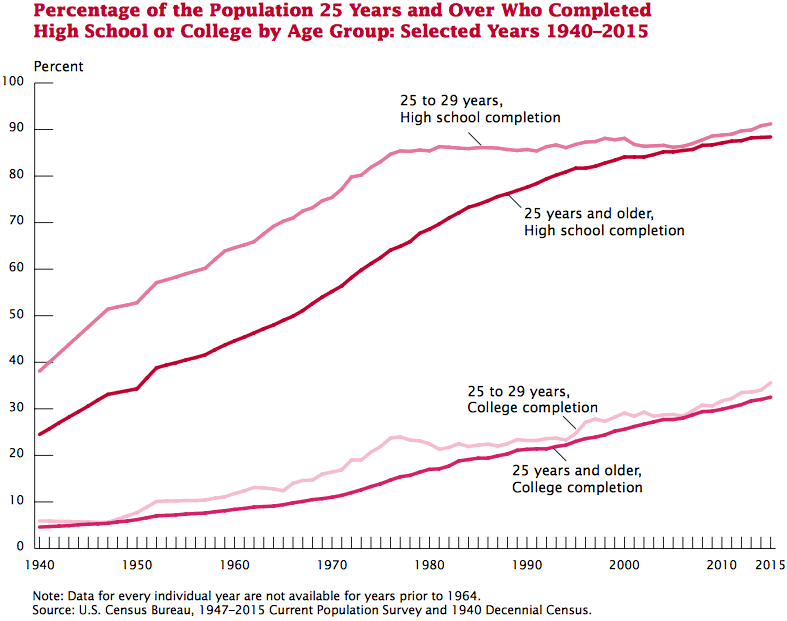
\includegraphics[keepaspectratio]{../images/9_educational_inequality.png}}

}

\caption{Educational Inequality in the U.S., 1940 to Present}

\end{figure}%

\paragraph{Occupation}\label{occupation}

Class is also composed of a person's \textbf{occupation}, or their paid
or unpaid employment. Occupations can obviously vary in terms of how
they are paid, but they also vary in terms of how much education they
require and how they are \emph{seen} by others (which is to say, the
status they carry).
\href{https://occupational-prestige.github.io/opratings/opratings.html}{This
website} provides a searchable ranking of occupational prestige using
data from the US Department of Labor. It shows that (again, somewhat
predictably) various kinds of Doctor and Lawyer rank the very highest,
while dishwashers rank the lowest. (If you're curious, ``sociologist''
ranks at 60.59 on a 100-point-scale, but substantially lower than the
rest of the ``Life, Physical, and Social Sciences'' field.)

\paragraph{The Controversial Element:
Lifestyle}\label{the-controversial-element-lifestyle}

The controversial component of class is \textbf{lifestyle}. This
comprises what people consume, how they are educated, who they associate
with, and even the kinds of cultural judgments they make. For instance,
the sociologist Anette Lareau (Lareau
2011)\marginpar{\begin{footnotesize}
\begin{CSLReferences}{2}{0}
\bibitem[\citeproctext]{ref-lareauUnequalChildhoodsClass2011}
Lareau, Annette. 2011.
\emph{\href{https://books.google.com?id=MK0GTCFvk8IC}{Unequal
{Childhoods}: {Class}, {Race}, and {Family Life}}}. University of
California Press.
\end{CSLReferences}
\vspace{2mm}\par\end{footnotesize}}
found that children from different class backgrounds were socialized to
two very different ``styles'' of interacting with intstitutions.
Children from working-class backgrounds were socialized into the
\emph{the accomplishment of natural growth}, which emphasized
comparatively little structured play and fostered relatively little
experience in challenging adverse decisions by authorities. The
\emph{concerted cultivation} practiced by middle-class families,
meanwhile, socialized children into highly-structured institutional play
(such as music lessons, camps, and so on) while teaching them to
question and challenge decisions they disagreed with.

There is also some evidence that these lifestyle differences extend to
cultural taste. Consider the following table, which shows the percentage
of respondents who like or dislike classical music accoding to their
``subjective'' (i.e., self-assessed) class. As you can see, the appeal
of classical music rises with class position, and distaste for it rises
class falls.

\begin{longtable}[]{@{}
  >{\centering\arraybackslash}p{(\linewidth - 8\tabcolsep) * \real{0.2857}}
  >{\centering\arraybackslash}p{(\linewidth - 8\tabcolsep) * \real{0.1688}}
  >{\centering\arraybackslash}p{(\linewidth - 8\tabcolsep) * \real{0.1948}}
  >{\centering\arraybackslash}p{(\linewidth - 8\tabcolsep) * \real{0.1818}}
  >{\centering\arraybackslash}p{(\linewidth - 8\tabcolsep) * \real{0.1688}}@{}}
\caption{Appeal of Classical Music by Subjective Class, General Social
Survey}\tabularnewline
\toprule\noalign{}
\begin{minipage}[b]{\linewidth}\centering
\end{minipage} & \begin{minipage}[b]{\linewidth}\centering
Lower Class
\end{minipage} & \begin{minipage}[b]{\linewidth}\centering
Working Class
\end{minipage} & \begin{minipage}[b]{\linewidth}\centering
Middle Class
\end{minipage} & \begin{minipage}[b]{\linewidth}\centering
Upper Class
\end{minipage} \\
\midrule\noalign{}
\endfirsthead
\toprule\noalign{}
\begin{minipage}[b]{\linewidth}\centering
\end{minipage} & \begin{minipage}[b]{\linewidth}\centering
Lower Class
\end{minipage} & \begin{minipage}[b]{\linewidth}\centering
Working Class
\end{minipage} & \begin{minipage}[b]{\linewidth}\centering
Middle Class
\end{minipage} & \begin{minipage}[b]{\linewidth}\centering
Upper Class
\end{minipage} \\
\midrule\noalign{}
\endhead
\bottomrule\noalign{}
\endlastfoot
Like It Very Much & 2\% & 37\% & 51\% & 8\% \\
Like It & 4\% & 43\% & 50\% & 3\% \\
Mixed Feelings & 5\% & 42\% & 49\% & 3\% \\
Dislike It & 9\% & 58\% & 31\% & 1\% \\
Dislike It Very Much & 10\% & 51\% & 38\% & 1\% \\
\end{longtable}

\section{Theories of Stratification and
Class}\label{theories-of-stratification-and-class}

There are a multitude of theories of class and stratification in
sociology, and we will touch on a few of the most important.

\subsection{Marx}\label{marx}

One of the most important theories of class and stratification in
sociology was developed by Karl Marx. Marx thought that one's class
position was defined by one's relationship to the \textbf{means of
production}, or the machinery necessary to actually produce what is
necessary to survive and live in modern societies. Some people in
society, called the \textbf{bourgeoisie} or \textbf{capitalists}, owned
the means of production. Under capitalism, Marx thought, the vast bulk
of society was made up of \textbf{workers} or the \textbf{proletariat},
which sells their own labor power as though it is a commodity (this is
what a ``wage'' is---the price your labor is worth on the market of
labor power).

A key dynamic of capitalism, according to Marx, was that inequality
would worsen under capitalism, concentrating wealth in the hands of
capitalists and progressively immiserating the proletariat. Marx
(mistakenly, as it happens) thought that this dynamic would inevitably
lead to a global worker-led revolution which would institute communism.
But what \emph{has} been validated by careful analysis (conducted by an
economist) is the observation that, in the absence of regulation,
inequality worsens under capitalism (Piketty
2017)\marginpar{\begin{footnotesize}
\begin{CSLReferences}{2}{0}
\bibitem[\citeproctext]{ref-pikettyCapitalTwentyfirstCentury2017}
Piketty, Thomas. 2017. \emph{Capital in the Twenty-First Century}.
Cambridge, Massachusetts London: The Belknap Press of Harvard University
Press.
\end{CSLReferences}
\vspace{2mm}\par\end{footnotesize}}.

\subsubsection{E. O. Wright}\label{e.-o.-wright}

In addition to the failures of Marxist theory to predict the outcome of
capitalist dynamics (one of its avowed goals), the theory has also been
modified to address another empirical drawback. As you might have
noticed in the above description, Marx's theory argues that there is an
austere gap between capitalists and workers. Yet, if we examine the
contemporary landscape of work in the U.S., we find that a multitude of
workers either have aspects of management in their work, perhaps own
their own small business and still work, or (even more frequently)
depend on retirment income on stocks and bonds, which make them (very
small scale and indirect) capitalists. The sociologist Erik Olin Wright
recognized and analyzed these \textbf{contradictory class locations},
and noted that they were becoming more widespread in contemporary
capitalism, and that they complicated the dynamics if capitalist change
(Wright
1985)\marginpar{\begin{footnotesize}
\begin{CSLReferences}{2}{0}
\bibitem[\citeproctext]{ref-wrightClasses1985}
Wright, Erik Olin. 1985. \emph{Classes}. London: Verso.
\end{CSLReferences}
\vspace{2mm}\par\end{footnotesize}}.

\subsection{Functionalists}\label{functionalists}

If Marxism sees conflict among classes with competing interests as the
central dynamic of society, functalists tend to emphasize social order.
Accordingly, a functionalist theory of inequality emphasizes the
``necessity'' of inequality (Davis and Moore
1945)\marginpar{\begin{footnotesize}
\begin{CSLReferences}{2}{0}
\bibitem[\citeproctext]{ref-davisPrinciplesStratification1945}
Davis, Kingsley, and Wilbert E. Moore. 1945. {``Some {Principles} of
{Stratification}.''} \emph{American Sociological Review} 10(2):242--49.
doi:\href{https://doi.org/10.2307/2085643}{10.2307/2085643}.
\end{CSLReferences}
\vspace{2mm}\par\end{footnotesize}}.
This is primarily because society ``needs'' to differentially reward
people who perform tasks that are more ``valuable'' for overall social
orders, and these rewards are evidence (tautologically) of those tasks'
increased importance.

\subsection{Weber}\label{weber}

Marx and the structural functionalists overwhelming concentrate on
\emph{economic} factors when thinking about class. The sociologists Max
Weber, however, recognized that class was also a composite of
\textbf{social status}, or the ways that people evaluate the positions
and esteem of others in a society. Weber argued that this different axis
of inequality created social positions (for instance, the clergy) that
did not neatly fit into the capitalist/worker distinction. Additionally,
the invocation of identity and meaning entails that some social
positions among ``workers'' might be accorded very different statuses
and, therefore, mean that people occupying them might have very
different identities. For instance, skilled tradesmen might not
necessarily see themselves as natural allies of unskilled laborers,
managers might not identify with capitalists, and so on.

\subsection{Bourdieu}\label{bourdieu}

Finally, Pierre Bourdieu, in his monumental \emph{Distinction}
(1984)\marginpar{\begin{footnotesize}
\begin{CSLReferences}{2}{0}
\bibitem[\citeproctext]{ref-bourdieuDistinctionSocialCritique1984}
Bourdieu, Pierre. 1984. \emph{Distinction: {A Social Critique} of the
{Judgement} of {Taste}}. Cambridge: Harvard University Press.
\end{CSLReferences}
\vspace{2mm}\par\end{footnotesize}}
argued that there was yet another neglected dimension of inequality and
class, which he named \textbf{cultural capital.} One of the crucial
theorists of ``lifestyle'' and class discussed above, Bourdieu argued
that cultural captial was the ability of people not only to make
judgments themselves, but also to claim that those judgments are
authoritative and legitimate. For instance, in the case of art, ``high
art'' wasn't just reducible to who had the money to pay for art, but
rather to a special class of \emph{critics} who were recognized with the
ability to distinguish between ``good art and bad.'' Crucially, this
rarely correlated directly with other markers of class, but observed a
dynamic all its own.

\section{Class in the United States}\label{class-in-the-united-states}

\subsection{Prologue: Measuring
Poverty}\label{prologue-measuring-poverty}

It is surprisingly difficult to measure poverty. One reason for this is
because to be ``poor'' is to be poor \emph{relative to some standard.}
At a basic level there are two such standards, and each standard has its
own measure of poverty.

The first of these is \textbf{absolute poverty}, which measures poverty
according to the costs of fulfilling basic life needs. This is the
standard used by the federal government, which sets the ``poverty line''
at three times the assumed cost of a nutritionally-adequate diet per
person. (This means that,
\href{https://aspe.hhs.gov/sites/default/files/documents/b1bfa16b20ae9b89d525bc35de7c1643/detailed-guidelines-2026.pdf}{in
2026}, the poverty line for a single person, excluding Hawaii and
Alaska, is 15,960 dollars a year. That's \textasciitilde\$43.72 a
day.)\sidenote{\footnotesize Note also that this aboluste poverty measure is
  \emph{not} regionally or cost-of-living adjusted (except for AK and
  HI)!}

The second standard is poverty is measured relative to the standards of
mainstream society, and is thus called \textbf{relative poverty.} Why
use this measure? Simply, there is now lots of evidence that
\emph{feeling} poor relative to the rest of society has numerous poor
effects on one's life, including on people's physical and mental health
(Pickett and Wilkinson
2008)\marginpar{\begin{footnotesize}
\begin{CSLReferences}{2}{0}
\bibitem[\citeproctext]{ref-pickettHealthInequality2008}
Pickett, Kate, and Richard G. Wilkinson. 2008.
\emph{\href{https://books.google.com?id=djdytAEACAAJ}{Health and
{Inequality}}}. Routledge.
\end{CSLReferences}
\vspace{2mm}\par\end{footnotesize}}.

\subsection{A Map of Class in the United
States}\label{a-map-of-class-in-the-united-states}

The upper-class in the US is composed of families making more than about
\$250,000 a year, is made of people who attended elite educational
institutions, and whose wealth mostly comes from investment dividends.
They comprise about 5\% of the US.

The middle class, meanwhile, is (in the U.S.) a notoriously amorphous
group comprising about 55\% of society. Incomes range from \$125,000 to
\$250,000 for the ``upper middle class'', who are usually
highly-education professionals, and between \$60,000 and \$125,000 for
the ``middle middle class,'' working in occupations like skilled crafts
and less-educated office workers.

Below the middle class stands the ``working class,'' which is about 20\%
of the U.S. class structure, and is composed of less-skilled
tradespeople and office workers, and whose income ranges from about
\$30,000 to \$60,000.

Finally, the ``lower class'' are people who work full time at low wages
(usually in retail or service work), part time, or not at all. They are
about 20\% of households, and their income is usually below \$30,000.

\subsection{Some Consequences: Class
Matters}\label{some-consequences-class-matters}

Our assigned reading for this unit, ``Class Matters,'' explores the
consequences of class on three New Yorkers (each from a different class)
who had the same kind of heart attack.

The first, a high-class architect, is surrounded by friends who identify
his heart attack immediately, receives the highest-quality care
immediately, and is able to retire on favorable terms early from his
firm in order to concentrate on this recovery. As you might guess, his
health some time later is ``better than ever.''

The middle class case in the story arrives the hospital relatively
promptly, but for cost reasons, is only given the best treatment after
cheapter de-clotting drugs are tried first. He struggles to maintain a
positive diet, and while he is able to step back his physical
responsibilities at work, is not able to immediately retire. As the
story closes, his health is middling.

The lower-class case works as a janitor from Eastern Europe, and she
does not have her heart attack treated until well after it has taken
place (she tries the ``home remedy'' of a shot of vodka first), cannot
stop working, and must manage travel to and from medical appointments on
public transit, which can take hours. By the end of the story, again as
one might predict, her health is failing, and she has become a
``full-time patient.''

The point of this example is that it mimics a natural experiment: three
people have the same medical issue, and what (it seems) explains their
actual health outcomes is not a difference in their injuries, but rather
differences in their class positions, which determine the quality of
their care and their ability to concentrate on their recoveries.

\subsection{Afterword: ``Cultures of
Poverty''}\label{afterword-cultures-of-poverty}

One of the greatest controversies in contemporary society, given the
very high levels of relative poverty demonstrated in the U.S., is what
causes people to be poor. Observers note that a substantial group of
poor people \emph{do} work (about 1/3 of people 16 and older who fell
below the federal poverty line worked in the last year), and that
poverty is disproportionately black and latino. And, even in places
where poverty has substantially improved (such as among the elderly),
there are still large racial and gender gaps (black older women living
along are about ten times more likely to be poor as White married
elderly men).

In U.S. politics, one common response (comprising about a third of the
population) is that the poor---and especially, the \emph{racialized}
poor---do not work sufficiently hard to lift themselves out of
poverty.\sidenote{\footnotesize The survey question was: ``On the average Black people
  have worse jobs, income, and housing than white people. Do you think
  these differences are\ldots Because most Black people just don't have
  the motivation or will power to pull themselves up out of poverty?''
  \href{https://gssdataexplorer.norc.org/trends?category=Civil\%20Liberties&measure=racdif4_r1}{Source}}

\begin{figure}[H]

{\centering \pandocbounded{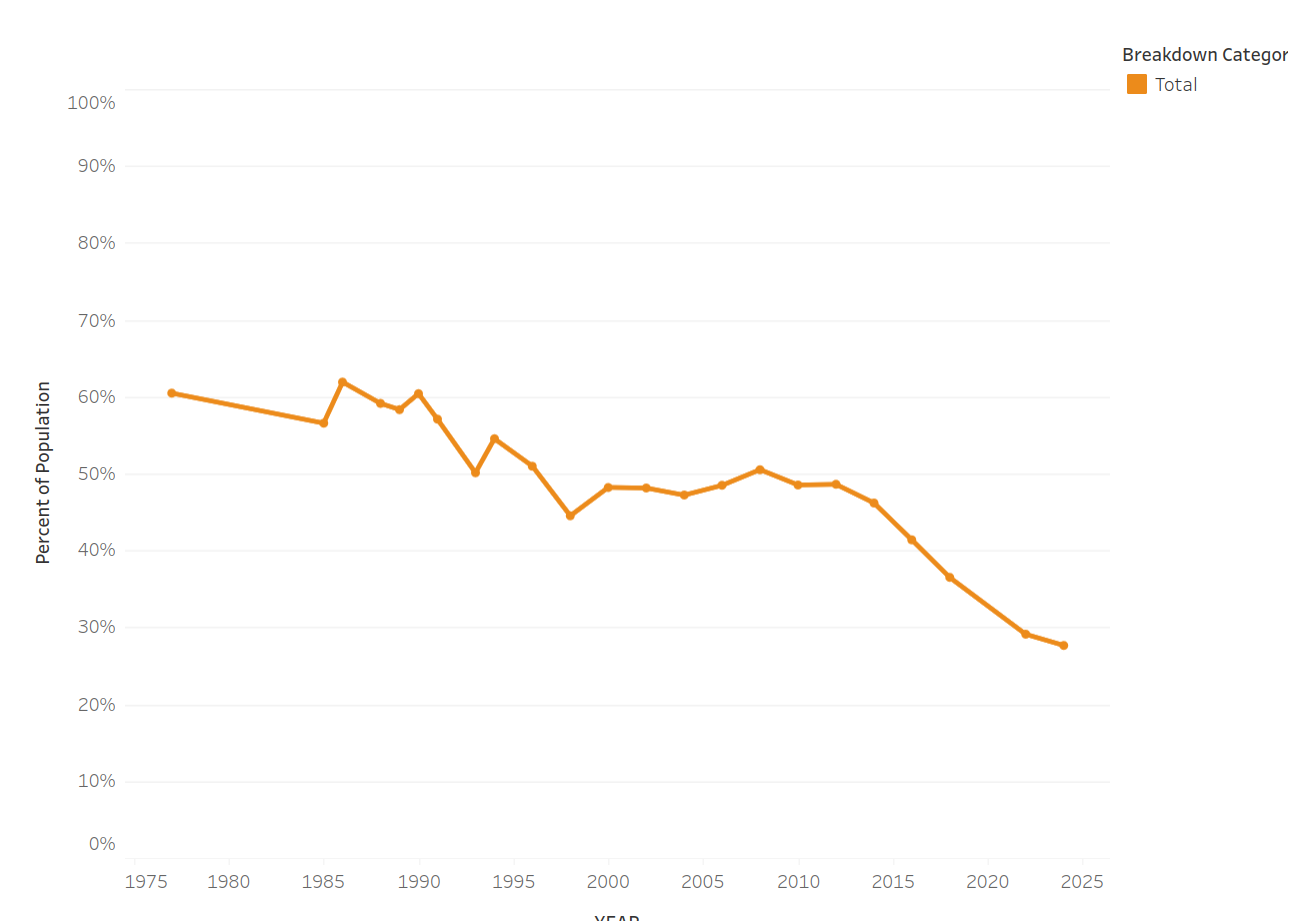
\includegraphics[keepaspectratio]{../images/9_black_poverty.png}}

}

\caption{Proportion of U.S. Population Ascribing Black Poverty to Lack
of Will Over Time}

\end{figure}%

In a more sanitized vocabulary, these arguments also exist in the social
sciences. Broadly, the competing poles argue, on the one hand, that
poverty happens because of structural factors out of the control of any
individual or subculture. On the other hand, some social scientists
argue that there \emph{are} specific cultural factors (whether it is
socialization into a lack of effort, or to lack of knowledge of how to
save, and so on) that keep people poor.

\section{Some Notes on World Poverty}\label{some-notes-on-world-poverty}

Two major trends are observable regarding world poverty. The first is
temporal: poverty has fallen, by most measures, remarkably over the last
200 years.

\begin{figure}[H]

{\centering \pandocbounded{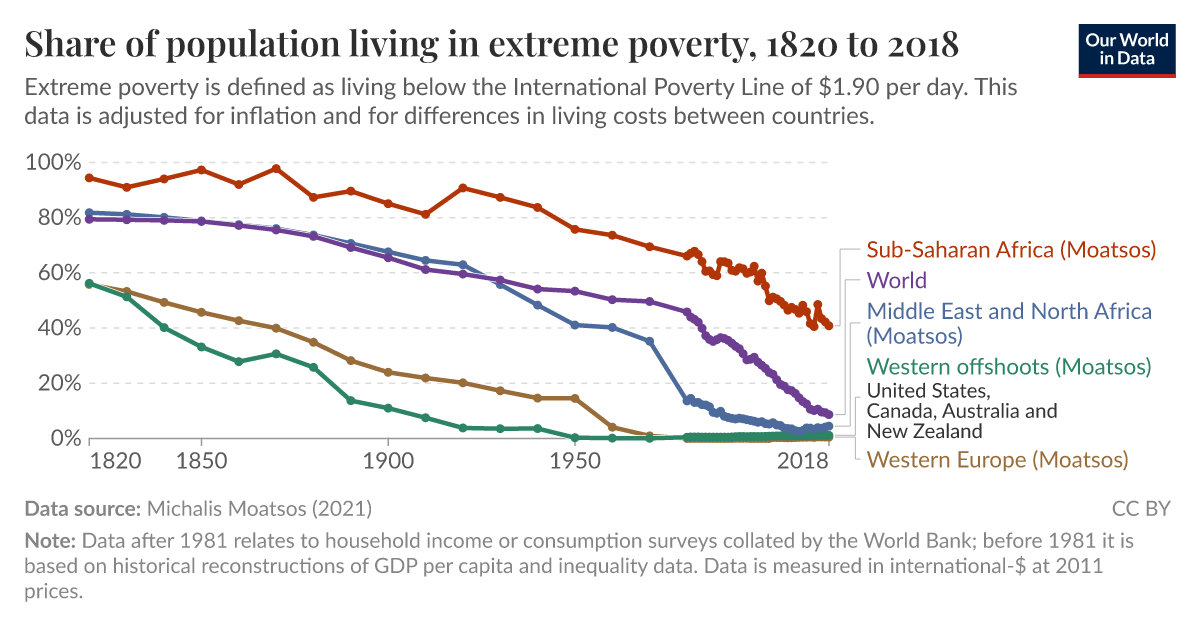
\includegraphics[keepaspectratio]{../images/9_poverty_over_time.png}}

}

\caption{Population Share in Extreme Poverty, 1820 to 2018}

\end{figure}%

Second, there is a high correlation between reduction in extreme
(absolute) poverty and the overall economic development of a country. As
economies on the whole become wealthy, there is almost no absolute
poverty, but as the economy on the whole is poorer, absolute poverty
increases.

\begin{figure}[H]

{\centering \pandocbounded{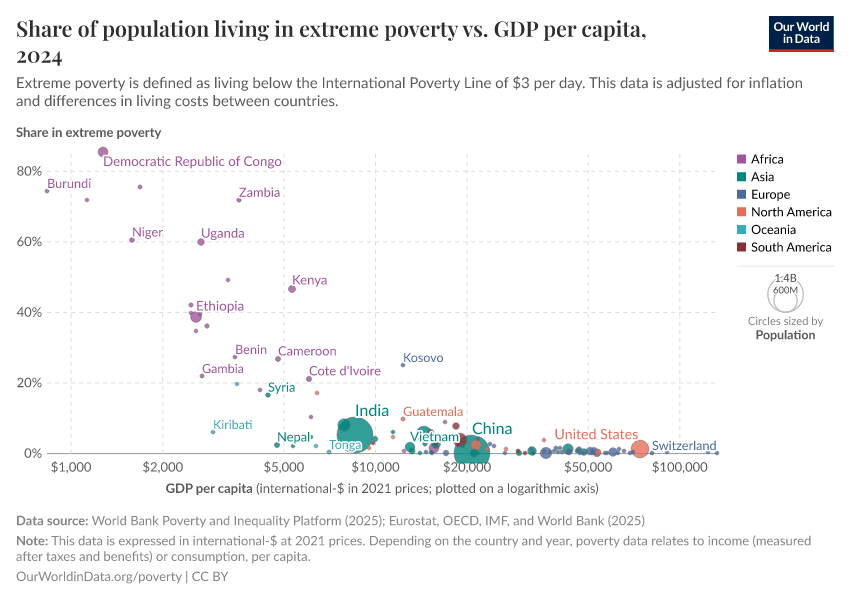
\includegraphics[keepaspectratio]{../images/9_global_poverty.png}}

}

\caption{Share of Population in Extreme Poverty, by Country, 2024}

\end{figure}%





\end{document}
